% Chapter 1

\chapter{Introduction} % Main chapter title
\thispagestyle{nohead}
\label{Intro} % For referencing the chapter elsewhere, use \ref{Intro} 

%----------------------------------------------------------------------------------------

% Define some commands to keep the formatting separated from the content 
\newcommand{\keyword}[1]{\textbf{#1}}
\newcommand{\tabhead}[1]{\textbf{#1}}
\newcommand{\code}[1]{\texttt{#1}}
\newcommand{\file}[1]{\texttt{\bfseries#1}}
\newcommand{\option}[1]{\texttt{\itshape#1}}
%----------------------------------------------------------------------------------------
The necessity of software verification (SV) has been demonstrated by numerous failures. 
Some of these failures have

Software faults can have disastrous consequences 
As the complexity of software projects increases

\section{Software Verification Background}
\subsection{Software Verification Systems as Composed of Modular Components}
\subsection{The \why~system}
\subsubsection{Front End: \why~as an intermediary language}
\subsubsection{Back End: Driver-based interface to \textsc{APT}, \textsc{ITP} and \textsc{SMT} tools}
\subsection{An overview of various \textsc{SMT} solvers and their capabilities}
\section{Problem Statement}

The efficient allocation of SMT-solving resources for software verification tasks

\section{Contributions}
The main contributions of this work are:
\begin{enumerate}
	\item The design  and implementation of our portfolio solver, \textsf{Where4}, which uses supervised machine learning to predict the best solver to use based on metrics collected from goals.
	\item The integration of \textsf{Where4} into the user's existing \textsf{Why3} work-flow by imitating the behaviour of an orthodox SMT solver.
	\item A set of metrics to characterise \textsf{Why3} goal formulae.
	\item Statistics on the performance of eight SMT solvers using a dataset of 1048 \textsf{Why3} goals.
	
\end{enumerate}

%\section{The benefits of a portfolio-based approach to software verification}
\begin{figure}
\centering
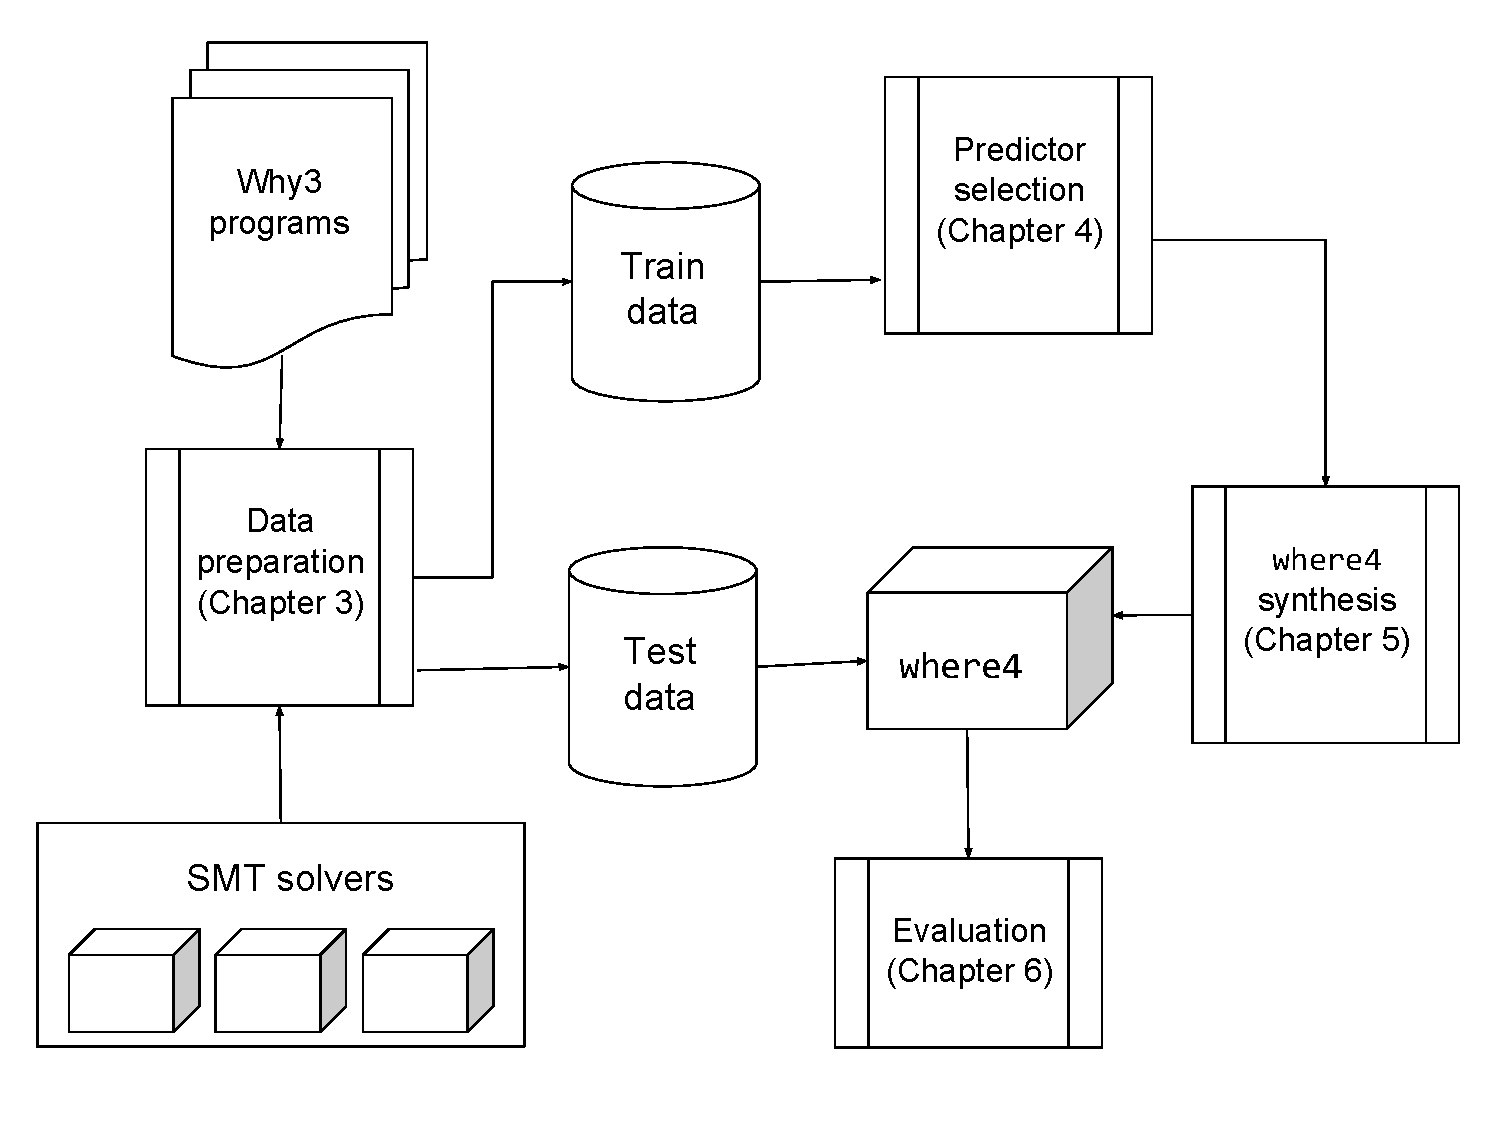
\includegraphics[width=0.9\linewidth]{Figures/intoduction}
\caption{Overview of the \where~project and this thesis's structure}
\label{fig:introduction}
\end{figure}

